
\section{Mapeo de Características}

Esta etapa del trabajo consiste en la implementación de un \textbf{mapa
de características} para la clasificación de las palabras según
la \textbf{categoría} que les fue asignada previamente.

Lo que se espera obtener es un \textbf{mapa auto-organizado} en el cual
cada \textbf{categoría} este claramente diferenciada.

Para lograr el objetivo presentaremos un \textbf{mapa auto-organizado} 
basado en el algoritmo de \emph{Kohonen}.

Detalleremos los pasos que realizamos para la implementación de la solución,
la elección de la implementación y las dificultades que nos topamos al
implementarlo.

Dividimos el informe en las siguientes secciones:

\begin{itemize}
\item Implementación del Algoritmo: detallamos de forma introductoria la
implementación del algoritmo. En las siguientes etapas discutiremos los pasos
hacia la implementación final.
\item Dimensiones Adecuadas: discutimos las alternativas para la dimensión
del mapa.
\item Vecindad, Learning Rate y Sigma: discutimos las alternativas que
estudiamos para seleccionar los parámetros.
\item 
\end{itemize}

\subsection{Implementación del Algoritmo}

Para implementar la solución tomamos el algoritmo de mapas
de \emph{Kohonen} visto en clase.

La versión que implementamos es la que realiza los calculos 
por \textbf{columna}, esta versión demora mas en los calculos 
que la versión matricial, pero su implementación nos resulto mas 
sencilla.

Tomamos una dimensíón del mapa de 20 x 20 y para la actualización 
de las vecindades utilizamos la \textbf{función gaussiana} con un 
\textbf{learning rate adaptativo}. Comenzando con un radio de 
vecindad de 10.

Para el entrenamiento utilizamos dos tipos de cota, una por \textbf{cantidad
de epocas} y la otra por \textbf{la diferencia de la norma de la matriz de pesos
entre dos epocas distintas}, cuando es menor a un delta se finaliza 
el entrenamiento.


\subsection{Dimensiones Adecuadas}

Buscamos una dimensión adecuada para el mapa, conociendo que queremos
clasificar 900 datos en 9 categorías.

Probamos con las siguientes dimensiones:

\begin{itemize}
	\item 10 x 10
	\item 20 x 20
	\item 30 x 30
\end{itemize}

\subsubsection{Dimensión 10 x 10 }

Obtuvimos que el mapa no era lo suficientemente grande y los valores de
entrada se solapaban mucho, como lo muestra la figura:

\begin{figure}[H]
  \centering
  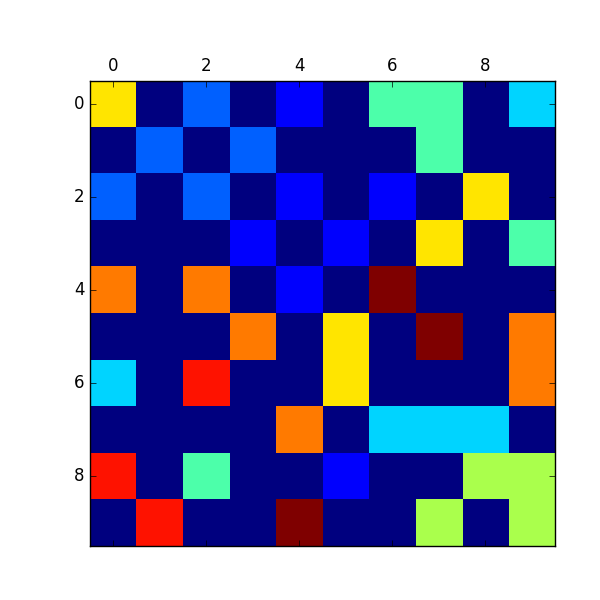
\includegraphics[width=0.8\columnwidth]{graficos/mapa1010.png}
  \caption{Mapa 10 x 10 para 200 entradas.}
  \label{fig:mapa 10 10 200}
\end{figure}


Por lo tanto descartamos esta configuración

\subsubsection{Dimensión 20 x 20 }

Con estas dimensiones obtuvimos una buena distribución de las categorías,
aunque hay un porcentaje de neuronas que no se activaron.

\begin{figure}[H]
  \centering
  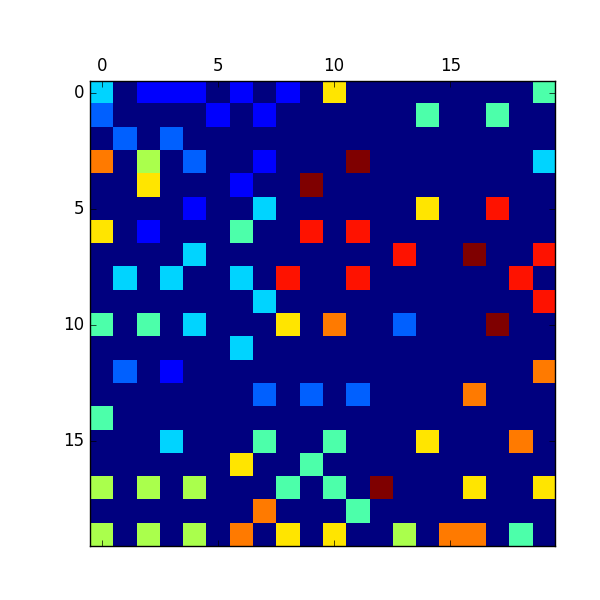
\includegraphics[width=0.8\columnwidth]{graficos/mapa2020.png}
  \caption{Mapa 20 x 20 para 200 entradas.}
  \label{fig:mapa 20 20 200}
\end{figure}


\subsubsection{Dimensión 30 x 30 }

Para esta configuración obtuvimos mayor desperdicio de neuronas,
es decir el porcentaje que nunca se activo fue muy alto, como lo muestra
la siguiente figura

\begin{figure}[H]
  \centering
  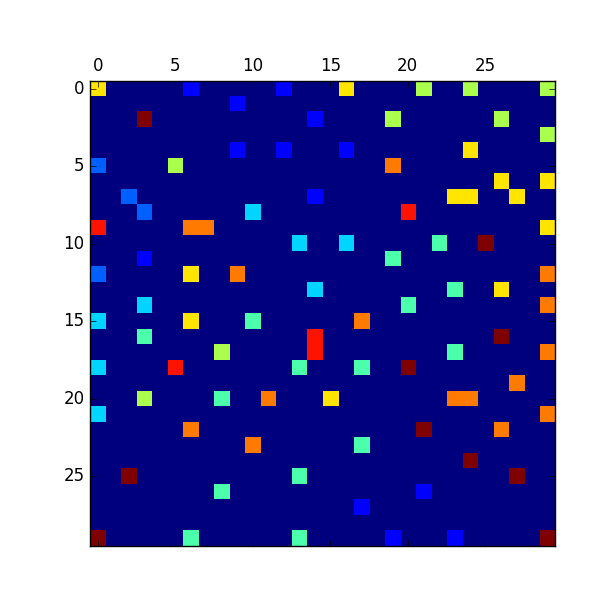
\includegraphics[width=0.8\columnwidth]{graficos/mapa3030.png}
  \caption{Mapa 30 x 30 para 200 entradas.}
  \label{fig:mapa 30 30 200}
\end{figure}


\subsubsection{Conclusión sobre la Dimensiones}


La que mejor se adapta a las características del problema, es la
de dimensión de 20 x 20.


\subsection{Vecindad, Learning Rate y Sigma}

Para la elección de estos parametros consideramos las siguientes
alternativas:

\textbf{Vecindad} por:

\begin{itemize}
	\item Escalones: influenciamos vecinos a distancia n formando
un cuadrado.
	\item Función Gaussiana: influenciamos n vecinos utilizando
una función gaussiana.
\end{itemize}


\textbf{Learning Rate} por:

\begin{itemize}
	\item Basado en la cantidad de epocas: definimos el learning
rate basado en la cantidad de epocas aplicadas a una función.
	\item Coeficientes adaptativos: definimos un valor de
learning rate inicial y lo disminuimos a traves de coeficientes.
	\item Decrecimiento porcentual: Definimos un valor de 
learning rate inicial y por epoca lo decrementamos en un 0.X por ciento.
\end{itemize}

Para el \emph{Learning Rate} basados en la \textbf{Cantidad de Epocas}, probamos con 
las siguientes funciones:

\begin{itemize}
	\item $\frac{1}{t^\frac{-1}{2}}$
	\item $\frac{1}{t^\frac{-1}{3}}$
\end{itemize}

En el caso de \textbf{Coeficientes Adaptativos}, probamos con:
$learning rate inicial / (1 + epoca_actual * coeficiente * learning rate inicial)$

Y para del \textbf{Decrecimiento Porcentual}: por cada epoca $learning rate inicial * 0.X$


\textbf{Sigma} por:

Definimos un valor de $sigma_inicial$, lo suficientemente grande para influenciar a todo 
el mapa. Y variandolo con las epocas con dos alternativas:

\begin{itemize}
	\item $sigmaInicial * {epocaActual^\frac{-1}{3}}$
	\item $sigmaInicial * e^\frac{epocaActual}{lambd}$
\end{itemize}

Tomando como lambd: $cantidadEpocas * cantidadDatosEntrenamiento / log(sigmaInicial)$


\subsubsection{Buscando la Combinación Ideal}

Realizamos una bateria de prueba tomando un set de datos de 300 valores, para
estudiar cual de la siguiente combinación de parametros organizaba mejor
las categorías.

Primero definimos un sigma inicial: (dimensión mapa) / 2, así en las primeras
epocas gran parte del mapa seria influenciado.

De las primeras pruebas concluimos que el \emph{Learning Rate} basado en la 
\textbf{cantidad de epocas} resultaba no ser una buena elección, ya que
decrece de forma muy rápido sin dar el tiempo suficiente para aprender.
Entonces descartamos esta opción.

Entonces utilizamos las otras dos opciones, definiendo un \emph{Learning Rate}
alto con valor de 0.999.En el caso de \textbf{Decrecimiento Porcentual}
tuvimos el inconveniente de que o decrecía muy rápido o demasiado lento, haciendo
dificil encontrar el punto justo.

El que nos permitió encontrar el balance fue \textbf{Coeficientes Adaptativos}
tomando como coeficiente = 0.5.

La función de \textbf{Sigma} basada en $sigmaInicial * e^\frac{epocaActual}{lambd}$
nos dió que decrecia de forma muy rápido, impidiendo el aprendizaje.
La función $sigmaInicial * {epocaActual^\frac{-1}{3}}$ combinado al \emph{Learning Rate}
de tipo \textbf{adaptativo} nos dió un buen balance.

Para la función de vecindad decidimos quedarnos con la \textbf{función uniforme} ya
que presentaba una distribución más ármonica.

\subsubsection{Conclusiones de los Parámetros}

La combinación que nos resulto mejor fue tomar:


\begin{itemize}
	\item $Sigma Inicial = 10$
	\item $Learning Rate Adaptativo = 0.999 / (1 + epoca_actual * 0.5 * 0.99)$
	\item $Sigma = Sigma Inicial * (epocaActual^\frac{-1}{3})$
\end{itemize}


\subsection{Cotas}

Para finalizar el entrenamiento definimos dos tipos de cotas:

\begin{itemize}
	\item Epocas
	\item Norma
\end{itemize}

La basada en la cantidad de \textbf{Epocas} establece una cantidad máxima de
ciclos de entrenamiento.

La basada en la \textbf{Norma} calcula la norma de la matriz de pesos (W) 
correspondiete a la epoca actual, hace la diferencia con la epoca anterior.
En caso que sea menor a una epsilon termina el entrenamiento. La ventaja
de esta es que cuando los pesos se modifican de forma despreciable entre
dos epocas significa que el aprendizaje comienza a estancarse.


\subsection{Entrenamiento}

Con los parametros seleccionados procedemos a realizar el entrenamiento de
nuestro mapa, para esto nos queda determinar la cantidad de datos con los que
conviene entrenar y estudiar si hay alguna diferencia variando las entradas
y las cotas con las que se finaliza el entrenamiento.

Tomamos distintos valores de entrada para entrenar, realizamos los test, y
reentrenamos el mapa nuevamente durante 3 etapas.

Con estas pruebas esperamos ver con que cantidad de datos de entrenamiento, 
con cual de las cotas y si la repetición influyen en la calidad de los resultados.

Al ingresar el parametro de entrenamiento, se toma una porción del dataset correspondiente
a la cantidad de entradas de forma random.


\subsubsection{50 Datos de Entrada}

\subsubsection{200 Datos de Entrada}

\subsubsection{800 Datos de Entrada}


\subsection{Detalles de Implementación}

La implementación de la solución fue desarrollada usando el lenguaje python,
con la librería numpy para facilitar las operaciones aritméticas y los gráficos
fueron construidos con la librería matplotlib.pyplot.

Para armar el mapa de Kohonen implementamos una clase \textbf{Kohonen} con la siguiente estructura:

\begin{lstlisting}
  struct kohonen {
    learning_rate = coeficiente de aprendizaje.
    tolerancia_error = cota de salida del entrenamiento para la diferencia entre normas.
    cantidad_epocas = cantidad máxima de epocas de entrenamiento.
    dimension = dimensión del mapa.
    entradas = cantidad de archivos usados para entrenar.
    input_file = archivo de entrada del dataset.
    data_entrenamiento = inicializado en 0.
    data_validacion = inicializado en 0.
    N = fijo en 856
    M1 = M2 = dimensión de entrada
    M = M1* M2 
    W = matriz de pesos inicializada en random.  
    cant_categorias = fijo en 9
    Mres = resultado de las categorias, inicializado en 0
    actualizarDataSet() = toma valores de entrada random segun la cantidad de entradas
  }
\end{lstlisting}

Para ejecutar el algoritmo correr: python ejercicio2.py

Para acceder al menú de ayuda ingresar: help

Para iniciar un entrenamiento ingresar: train

Para validar los datos ingresar: test

Para guardar los resultados de entrenamiento ingresar: export nombreMapa.in

Para importar un mapa ingresar import nombreMapa.in

Para salir del programa ingresar: exit


\subsection{Detalles de Resultados}

Los resultados correspondientes a la sección de entrenamiento son adjuntados con 
la siguiente estructura:

XXX Entradas/Etapa X/: la carpeta Entradas corresponde a la cantidad de datos usados para entrenar la red
y la subcarpeta Etapa corresponde a una etapa de entrenamiento. Dentro de la carpeta de
Etapas se encuentran los siguientes archivos

\begin{itemize}
	\item mapa XXX X.in =  corresponde al mapa entrenado.
	\item resultados mapa XXX X.txt = corresponde a los resultados de ejecutar la
validación sobre el entrenamiento.
	\item mapa XXX X aciertos.png = muestra la posición en la mapa de los registros bien clasicados.
	\item mapa XXX X errores.png = muestra la posición en la mapa de los registros mal clasicados.
	\item mapa XXX X indefinidas.png = = muestra la posición en la mapa de los registros que no
se han podido clasificar.
	\item mapa XXX X entrenamiento = es el mapa obtenido del entrenamiento.
\end{itemize}

\subsection{Conclusiones}

